\chapter{Système d'exploitation}

\section{Splash screen}

Le système d'exploitation disposait déjà d'un écran de démarrage aux couleurs de l'école survenant lors de la phase d'initialisation du système.

Un second a été ajouté lors de la phase précédente, le démarrage du kernel, c'est à dire de Linux. Cela n'a pas vraiment d'intérêt pour le télescope si ce n'est un peu d'esthétique lorsqu'il démarre avec un écran branché. Cependant cela met en œuvre un processus qui sera utile pour d'autres choses, la configuration du kernel.

\vspace{1cm}

Les éléments des sources de Linux impliqués dans le splash screen sont les suivants~:
\begin{itemize}[label=$\bullet$]
	\item Dans le dossier \codeinline{text}{kernel-source/drivers/video/logo/}
	\begin{itemize}
		\item \codeinline{text}{Makefile}
		\item \codeinline{text}{Kconfig}
		\item \codeinline{text}{logo.c}
		\item Différents fichiers image, ceux nous intéressant sont au format \codeinline{text}{logo_*_clut224.ppm}
		\end{itemize}
	\item Dans le dossier \codeinline{text}{kernel-source/include/linux/}
	\begin{itemize}
		\item \codeinline{text}{linux_logo.h}
		\end{itemize}
	\end{itemize}

\vspace{1cm}

Tout d'abord l'on crée une recette yocto de surcharge de la recette kernel utilisée par la \codeinline{text}{meta-raspberrypi}. Voici l'allure du dossier associé à la recette. À noter que l'arborescence utilisée par une recette de surcharge du kernel est plus sensible qu'une recette de surcharge quelconque.

\code{text}
~/yocto/sources/meta-autoscope $ tree recipes-kernel/
    recipes-kernel/
    └── linux/
        ├── linux-raspberrypi/
        │   └── raspberrypi3/
        └── linux-raspberrypi_%.bbappend
\end{minted}

\vspace{1cm}

Ensuite l'on crée l'image qui servira d'écran de démarrage, en commencant par lui donner les dimensions souhaitées, ici $1822\times 900$. Il faut alors la convertir au format qui convient~:

\code{text}
jpegtopnm lune-1822x900.jpg | ppmquant 224 | pnmnoraw > logo_autoscope_clut224.ppm 
mv logo_autoscope_clut224.ppm ~/yocto/sources/meta-autoscope/recipes-kernel/linux/linux-raspberrypi/raspberrypi3/
\end{minted}

\vspace{1cm}

Puis des lignes sont à ajouter dans les sources du kernel dont la localisation dans l'arborescence yocto est la suivante~:
\codeinline{text}{~/yocto/build/tmp/work-shared/raspberrypi3/kernel-source/}

\vspace{1cm}

\codeinline{text}{include/linux/linux_logo.h}~:
\code{C}
extern const struct linux_logo logo_autoscope_clut224;
\end{minted}

%\vspace{1cm}

\codeinline{text}{drivers/video/logo/logo.c}~:
\code{C}
#ifdef CONFIG_LOGO_AUTOSCOPE_CLUT224
        /* Autoscope Linux logo */
        logo = &logo_autoscope_clut224;
#endif
\end{minted}

%\vspace{1cm}

\codeinline{text}{drivers/video/logo/Makefile}~:
\code{makefile}
obj-$(CONFIG_LOGO_AUTOSCOPE_CLUT224)    += logo_autoscope_clut224.o
\end{minted}

%\vspace{1cm}

\codeinline{text}{drivers/video/logo/Kconfig}~:
\code{kconfig}
config LOGO_AUTOSCOPE_CLUT224
    bool "224-color Autoscope Linux logo"
    default y

\end{minted}

%\vspace{1cm}

On réalise un patch de ces modifications~:

\code{text}
~/yocto/build/tmp/work-shared/raspberrypi3/kernel-source $
    git add drivers/video/logo/{Kconfig,Makefile,logo.c} incude/linux/linux_logo.h
    git commit -m "Autoscope logo"
    git format-patch -1
    mv 0001-Autoscope-logo.patch ~/yocto/sources/meta-autoscope/recipes-kernel/linux/linux-raspberrypi/raspberrypi3/
\end{minted}

\vspace{1cm}

On configure ensuite le kernel afin d'activer l'écran de démarrage et de choisir celui souhaité. On réalise pour cela un $fragment$ de configuration~:

\codeinline{text}{meta-autoscope/recipes-kernel/linux/linux-raspberrypi/raspberrypi3/logo.cfg}~:
\code{C}
CONFIG_LOGO=y
CONFIG_LOGO_LINUX_MONO=y
CONFIG_LOGO_LINUX_VGA16=y
# CONFIG_LOGO_LINUX_CLUT224 is not set
CONFIG_LOGO_AUTOSCOPE_CLUT224=y
\end{minted}

\vspace{1cm}

La dernière étape est d'écrire la recette pour prendre en compte toutes ces modifications~:

\codeinline{text}{meta-autoscope/recipes-kernel/linux/linux-raspberrypi_\%.bbappend}~:
\code{bash}
FILESEXTRAPATHS_prepend := "${THISDIR}/${PN}:"

SRC_URI_append_raspberrypi3 += " \
    file://0001-Autoscope-logo.patch \
    file://logo.cfg \
    file://logo_autoscope_clut224.ppm \
    "

do_patch_prepend() {
    cp ${WORKDIR}/logo_autoscope_clut224.ppm ${S}/drivers/video/logo/
}
\end{minted}

\vspace{1cm}
Voici donc l'arborescence associée à la recette~:

\code{text}
~/yocto/sources/meta-autoscope $ tree recipes-kernel/
    recipes-kernel/
    └── linux/
        ├── linux-raspberrypi/
        │   └── raspberrypi3/
        │       ├── 0001-Autoscope-logo.patch
        │       ├── logo_autoscope_clut224.ppm
        │       └── logo.cfg
        └── linux-raspberrypi_%.bbappend
\end{minted}

\vspace{1cm}

Après une longue phase de compilation puisque le kernel est recompilé, on observe au démarrage la succession des deux écrans de démarrages~:

\begin{figure}[H]
    \centering
    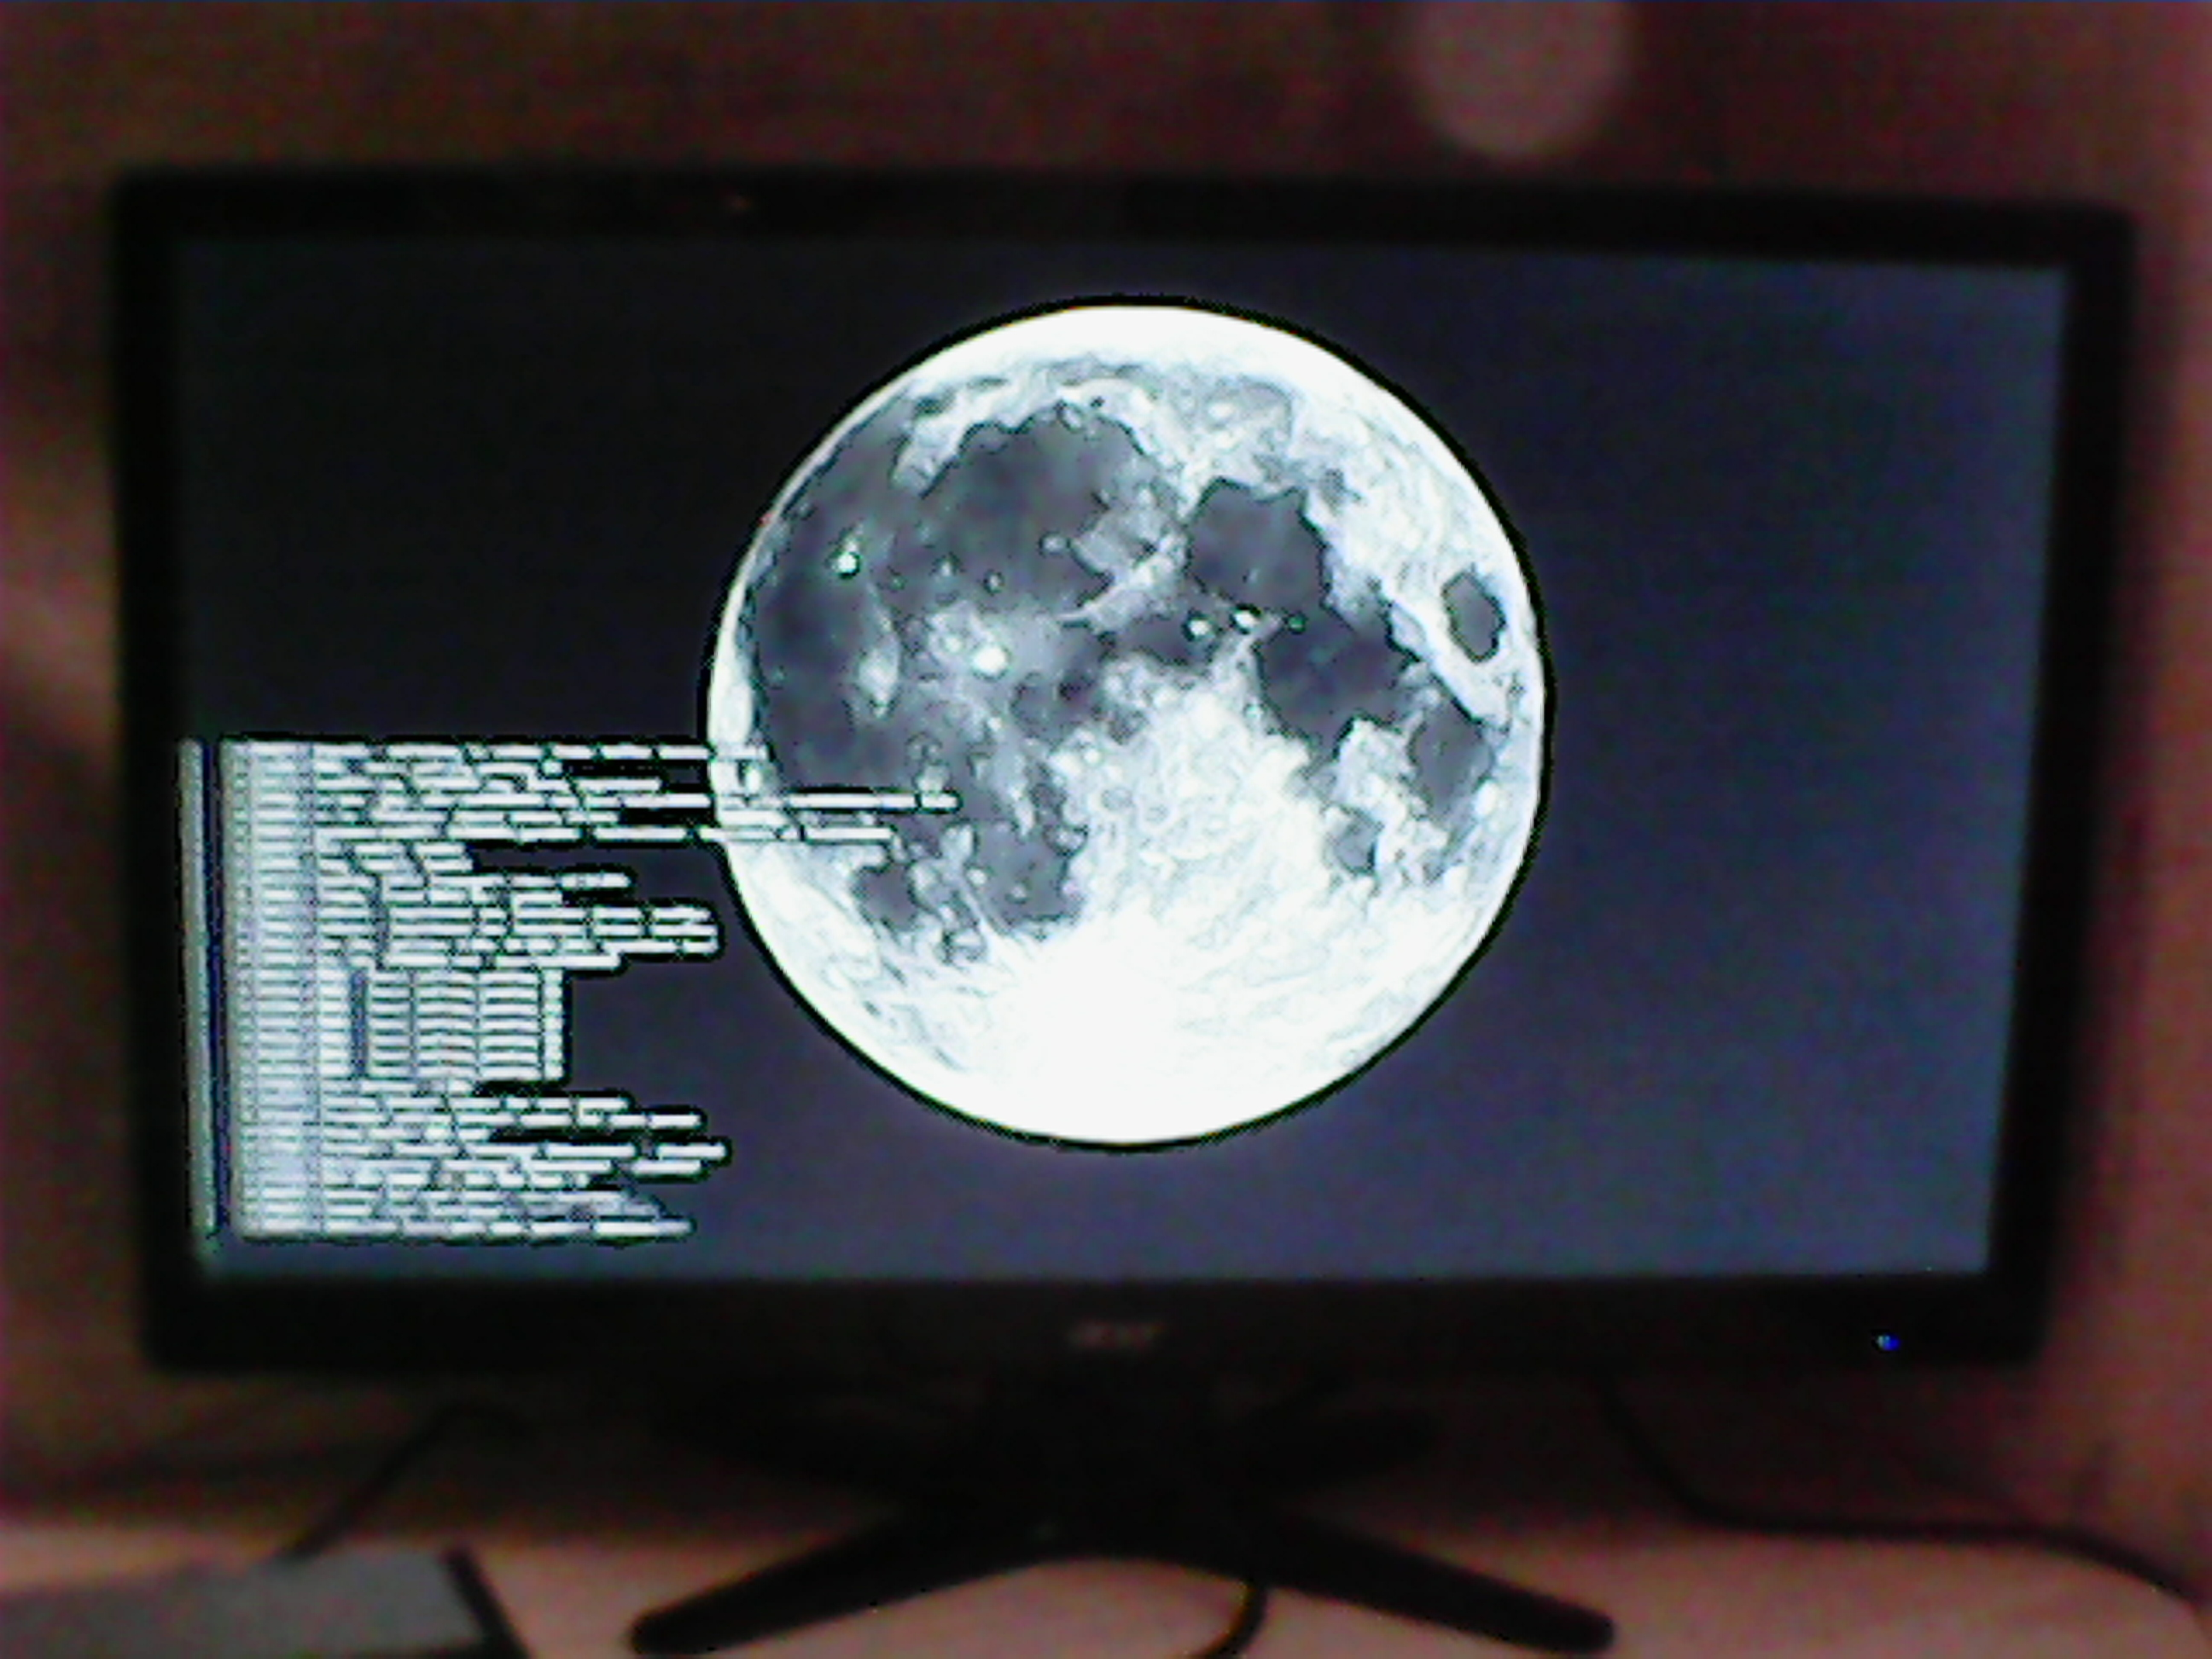
\includegraphics[width=0.49\linewidth]{\figures/photo_splashk_2.jpg}
    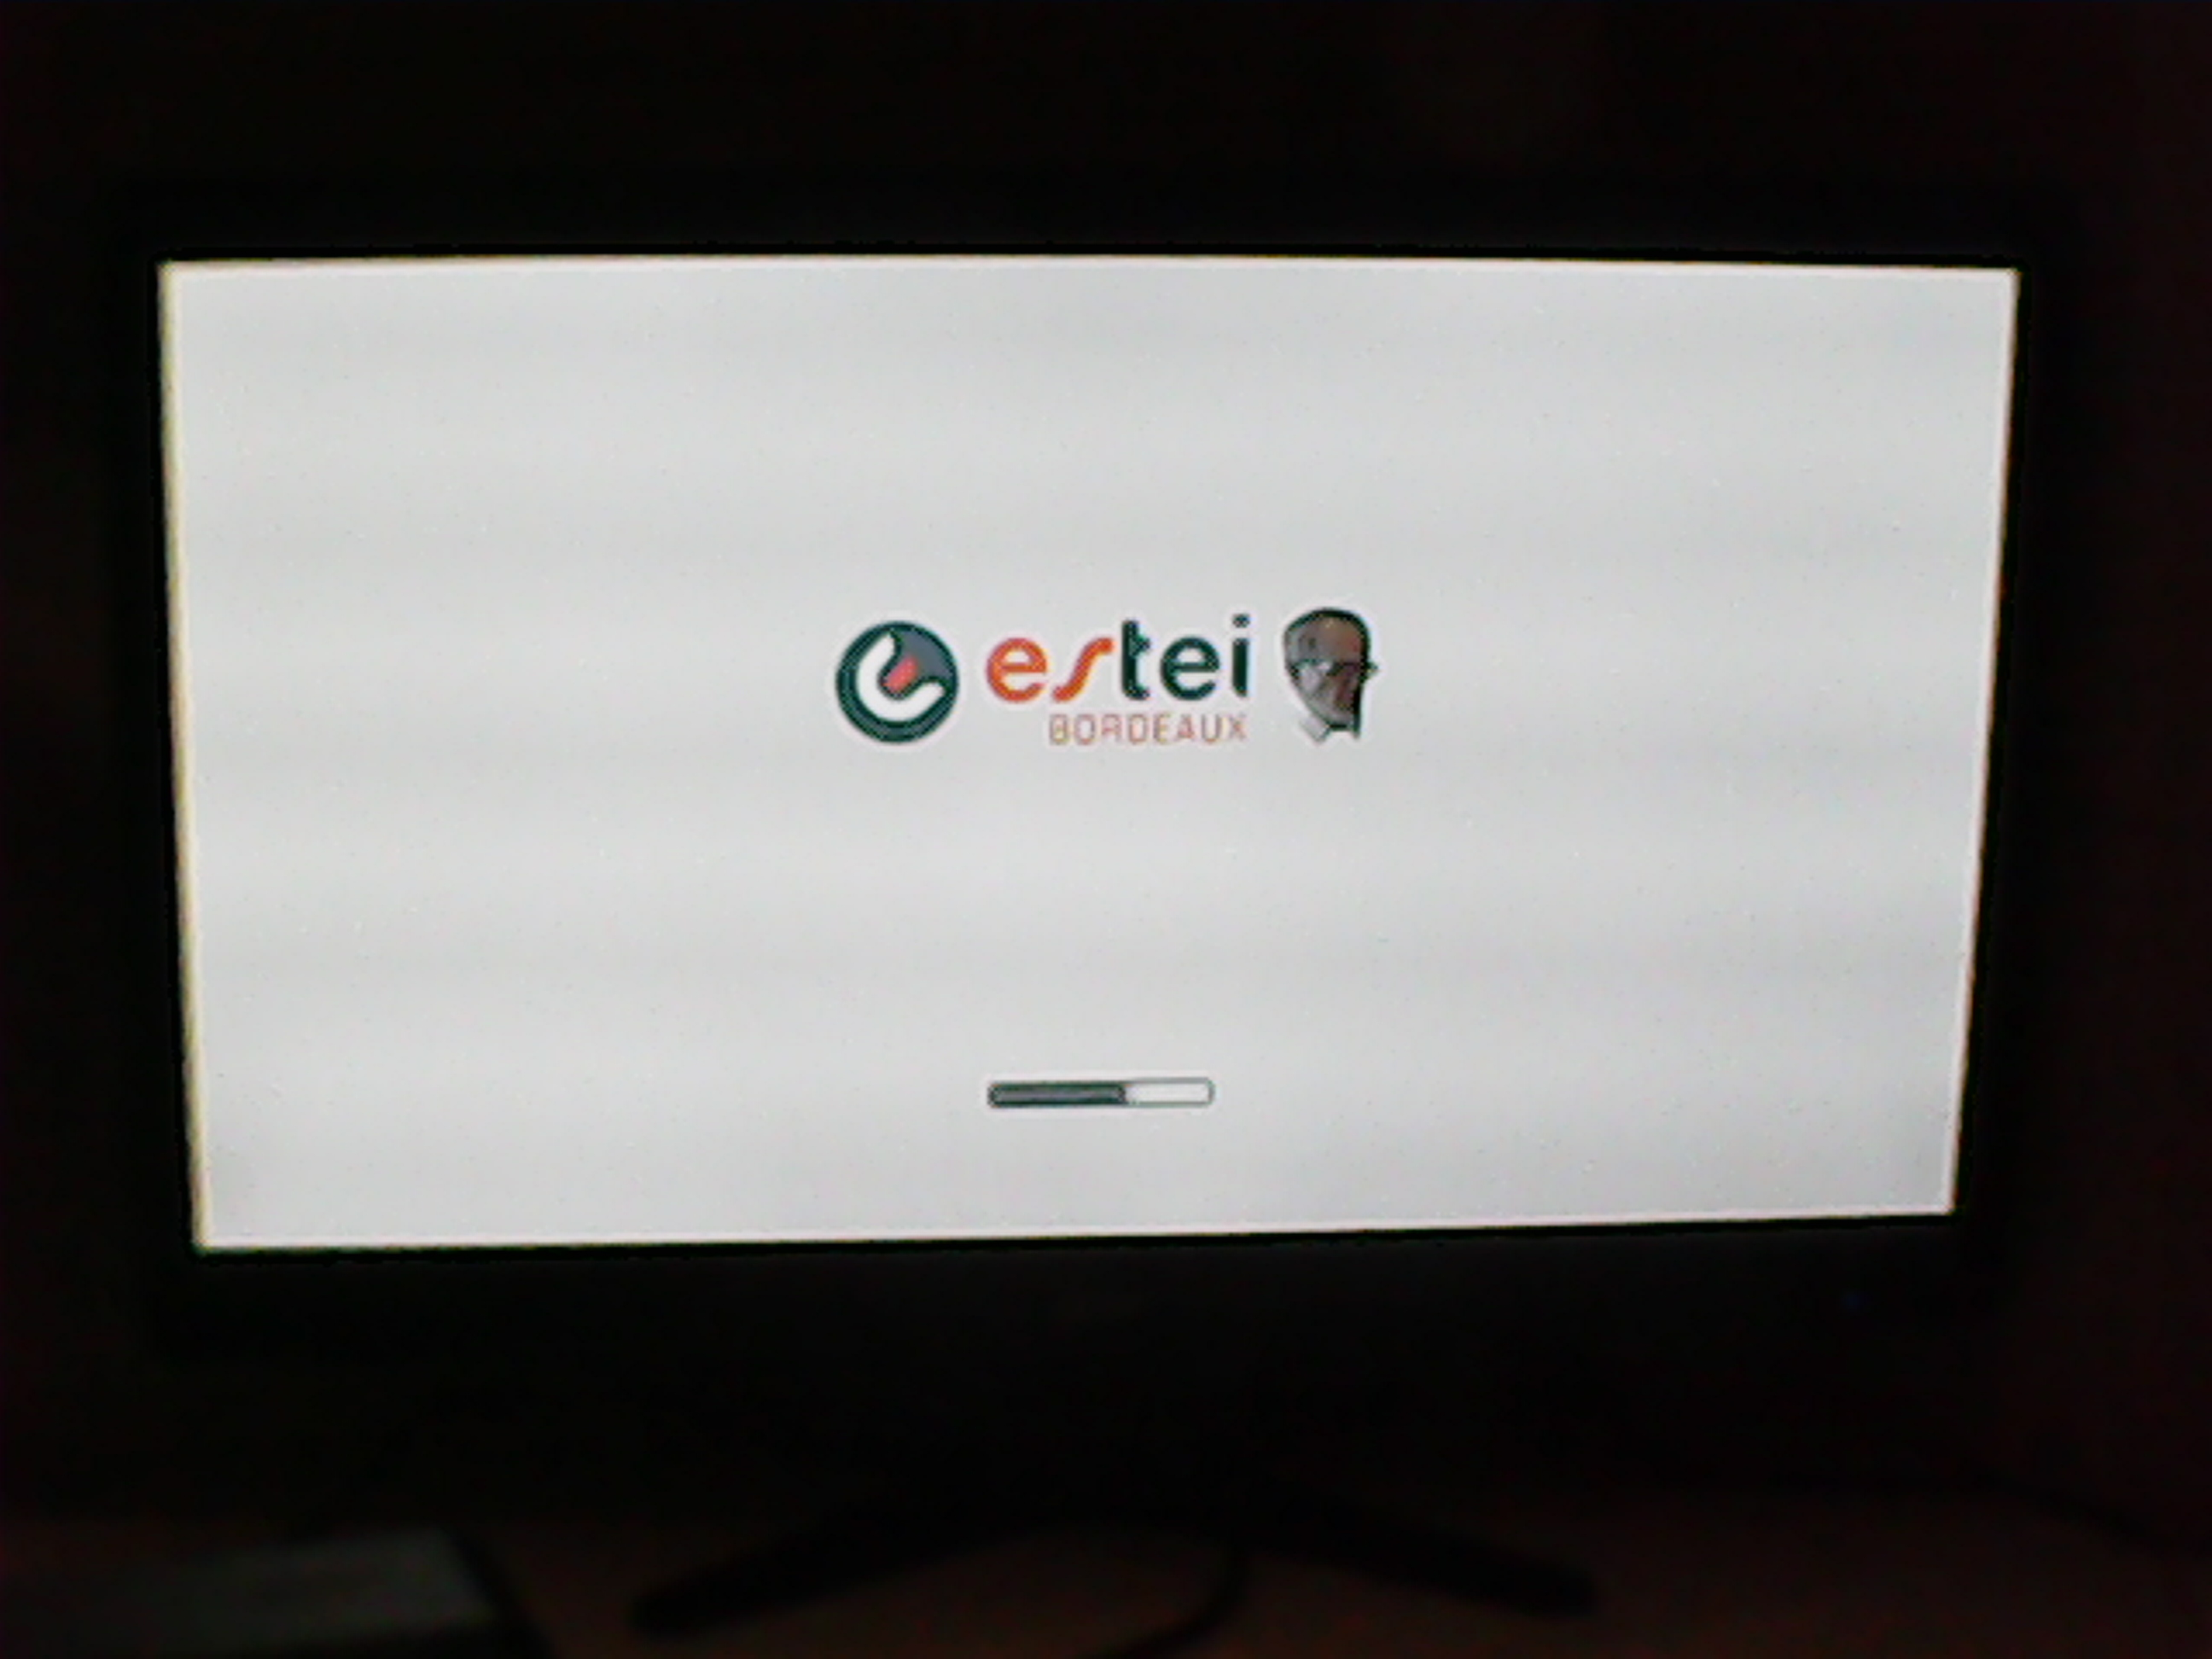
\includegraphics[width=0.49\linewidth]{\figures/photo_splashi_1.jpg}
    \decoRule
    \caption[
    Écrans de démarrage du noyau Linux à droite et du processus d'initialisation à gauche]{
    Écrans de démarrage du noyau Linux à droite et du processus d'initialisation à gauche}
    \label{fig:Écrans de démarrage du noyau Linux à droite et du processus d'initialisation à gauche}
    \end{figure}

\section{Hotspot Wifi}

Configurer le télescope en Hotspot Wifi est une solution intéressante car ainsi un appareil client peut s'y connecter sans qu'il n'y ait besoin d'une infrastructure existante, un réseau local par exemple.

Pour configurer la Raspberry-Pi en Hotspot, deux choses sont nécessaires~:
\begin{itemize}[label=$\bullet$]
	\item Configurer le kernel pour qu'il supporte le mode \codeinline{text}{tether}.
	\item Le logiciel \codeinline{text}{connman}
	\end{itemize}

\codeinline{text}{meta-autoscope/recipes-kernel/linux/linux-raspberrypi/raspberrypi3/hotspot.cfg}~:
\code{c}
CONFIG_BRIDGE=m
CONFIG_IP_NF_TARGET_MASQUERADE=m
CONFIG_NETFILTER=m
CONFIG_NF_CONNTRACK_IPV4=m
CONFIG_NF_NAT_IPV4=m

CONFIG_IP_NF_IPTABLES=m
CONFIG_IP_MULTIPLE_TABLES=m
CONFIG_NETFILTER_NETLINK_ACCT=m
CONFIG_NETFILTER_XT_MATCH_NFACCT=m
CONFIG_NETFILTER_XT_CONNMARK=m
CONFIG_NETFILTER_XT_TARGET_CONNMARK=m
CONFIG_NETFILTER_XT_MATCH_CONNMARK=m
\end{minted}

\codeinline{text}{meta-autoscope/recipes-kernel/linux/linux-raspberrypi_\%.bbappend}~:
\code{bash}
SRC_URI_append_raspberrypi3 += " \
    file://0001-Autoscope-logo.patch \
    file://logo.cfg \
    file://hotspot.cfg \
    file://logo_autoscope_clut224.ppm \
    "
\end{minted}

\codeinline{text}{meta-autoscope/recipes-autoscope/images/autoscope-console-image.bb}~:
\code{bash}
HOTSPOT = " \
    connman \
    connman-client \
    iptables \
"

IMAGE_INSTALL += " \
    ${CAMERA} \
    ${HOTSPOT} \
"
\end{minted}

\vspace{1cm}

Si l'on effectue les commandes suivantes, la Raspberry-Pi devient visible sur le réseau~:
\code{text}
root@autoscope ~ #
    sysctl -w net.ipv4.ip_forward=1
    connmanctl enable wifi
    connmanctl tether wifi on Autoscope 123456789
\end{minted}

\vspace{1cm}

Pour automatiser le processus au démarrage, il faut utiliser le paquet \codeinline{text}{connman-conf} et remplir quelques fichiers de configuration~:

\codeinline{text}{meta-autoscope/recipes-autoscope/images/autoscope-console-image.bb}~:
\code{bash}
HOTSPOT = " \
    connman \
    connman-client \
    connman-conf \
    iptables \
"
\end{minted}

\codeinline{text}{meta-autoscope/recipes-connectivity/connman-conf/files/main.conf}~:
\code{text}
[General]
DefaultAutoConnectTechnologies=wifi
TetheringTechnologies=true
PersistantTetheringMode=true
\end{minted}

\codeinline{text}{meta-autoscope/recipes-connectivity/connman-conf/files/settings}~:
\code{text}
[global]
OfflineMode=false

[WiFi]
Enable=true
Tethering=true
Tethering.Identifier=Autoscope
Tethering.Passphrase=123456789

[Wired]
Enable=true
Tethering=false

[P2P]
Enable=false
Tethering=false
\end{minted}

\codeinline{text}{meta-autoscope/recipes-connectivity/connman-conf/connman-conf.bbappend}~:
\code{bash}
FILESEXTRAPATHS_prepend := "${THISDIR}/files:"

SRC_URI += " \
    file://main.conf \
    file://settings \
"

FILES_${PN} += "${sysconfdir}/*"

do_install_append() {
    install -d ${D}${sysconfdir}/connman/
    install -m 0755 ${WORKDIR}/main.conf ${D}${sysconfdir}/connman/main.conf
    install -d ${D}${localstatedir}/lib/connman/
    install -m 0755 ${WORKDIR}/settings ${D}${localstatedir}/lib/connman/settings
}
\end{minted}

Les lignes ajoutées à \codeinline{text}{do_install()} permettent de déplacer les fichiers à leur place dans l'arborescence du système~:
\begin{itemize}[label=$\bullet$]
	\item \codeinline{text}{/etc/connman/main.conf}
	\item \codeinline{text}{/var/lib/connman/settings}
	\end{itemize}

\vspace{1cm}

À noter que sans la ligne \codeinline{text}{FILES_${PN} += "${sysconfdir}/*"}, Bitbake est incapable de connaître cette variable et donc de déplacer le fichier. La question ne se pose pas pour la variable \codeinline{text}{localstatedir} puisque l'on trouve la ligne suivante\\\codeinline{text}{FILES_${PN} = "${localstatedir}/* ${datadir}/*"} dans la recette originale~:\\\codeinline{text}{poky/meta/recipes-connectivity/connman-conf/connman-conf.bb}

\vspace{1cm}

Quant à la commande \codeinline{text}{sysctl -w net.ipv4.ip_forward=1} qui n'est pas à effectuer à chaque démarrage, on peut l'automatiser ainsi~:

\codeinline{text}{meta-autoscope/recipes-autoscope/images/autoscope-console-image.bb}~:
\code{bash}
hotspot() {
    echo 'net.ipv4.ip_forward = 1' >> ${IMAGE_ROOTFS}/etc/sysctl.conf
}

ROOTFS_POSTPROCESS_COMMAND += " hotspot; "
\end{minted}

\vspace{1cm}

Ainsi, dès le démarrage de la Raspberry-Pi, le Hotspot \codeinline{text}{Autoscope} est visible depuis un équipement Wifi. Le mot de passe est \codeinline{text}{123456789}.

Cela a fonctionné jusqu'à la mise en place de l'écran de démarrage qui passe également par une configuration du kernel. Un conflit doit exister mais n'a pas encore été repéré et arrangé.

\section{Serveur FTP}

Plusieurs serveurs FTP sont disponibles dans Poky, \codeinline{text}{vsftpd} semble être une bonne solution pour sa légèreté, sa fiabilité et ses possibilités de configuration.

\codeinline{text}{meta-autoscope/recipes-autoscope/images/autoscope-console-image.bb}~:
\code{bash}
FTP = " \
    vsftpd \
"

IMAGE_INSTALL += " \
    ${CAMERA} \
    ${HOTSPOT} \
    ${FTP} \
"
\end{minted}

\codeinline{text}{meta-autoscope/recipes-connectivity/vsftpd/vsftpd_\%.bbappend}~:
\code{bash}
FILESEXTRAPATHS_prepend := "${THISDIR}/files:"
\end{minted}

\codeinline{text}{meta-autoscope/recipes-connectivity/vsftpd/files/vsftpd.user_list}~:
\code{bash}
autoscope
\end{minted}

\codeinline{text}{meta-autoscope/recipes-connectivity/vsftpd/files/vsftpd.conf}~:
\code{bash}
listen=YES
anonymous_enable=NO
local_enable=YES
write_enable=YES
local_umask=022
dirmessage_enable=YES
xferlog_enable=YES
connect_from_port_20=YES
xferlog_std_format=YES
ftpd_banner=Welcome to Autoscope FTP service.
ls_recurse_enable=YES
pam_service_name=vsftpd
userlist_deny=NO
userlist_enable=YES
use_localtime=YES
chroot_local_user=YES
allow_writeable_chroot=YES
tcp_wrappers=YES
user_sub_token=$USER
local_root=/home/$USER
\end{minted}

Note~: Des commentaires explicatifs figurent dans le fichier \codeinline{text}{vsftpd.conf} mais ne sont pas affichés ici.

\vspace{1cm}

Le serveur est alors accessible depuis un navigateur web via l'URL \codeinline{text}{ftp://<ip.raspberry.pi>} ou plus simplement la commande \codeinline{text}{ftp autoscope@<ip.raspberry.pi>}. Le mot de passe de l'utilisateur \codeinline{text}{autoscope} est demandé.

\codeinline{text}{autoscope} est le seul utilisateur autorisé à accéder au serveur FTP.

De plus le serveur se lance automatiquement lors de la phase d'initialisation du système.

\section{Driver helloworld}

Ce driver minimaliste a pour but de préparer le terrain pour les drivers des moteurs, du GPS et de l'IMU.

\codeinline{text}{hello.c}~:
\code{C}
#include <linux/module.h>

int init_module(void)
{
    printk("Hello World!\n");
    return 0;
}

void cleanup_module(void)
{
    printk("Goodbye Cruel World!\n");
}

MODULE_LICENSE("GPL");
\end{minted}

\codeinline{text}{Makefile}~:
\code{makefile}
obj-m := hello.o

SRC := $(shell pwd)

all:
    $(MAKE) -C $(KERNEL_SRC) M=$(SRC)

modules_install:
    $(MAKE) -C $(KERNEL_SRC) M=$(SRC) modules_install

clean:
    rm -f *.o *~ core .depend .*.cmd *.ko *.mod.c
    rm -f Module.markers Module.symvers modules.order
    rm -rf .tmp_versions Modules.symvers
\end{minted}

Un fichier \codeinline{text}{COPYING} contient une licence GPL.

\vspace{1cm}

Tous ces fichiers figurent sur une branche dédiée \codeinline{text}{hello_mod} du dépôt~:\\\codeinline{text}{github.com/thibaudledo/Autoscope}.

\vspace{1cm}

\codeinline{text}{meta-autoscope/recipes-test/hello-mod/hello-mod_git.bb}~:
\code{bash}
SUMMARY = "Example of how to build an external Linux kernel module"
LICENSE = "GPLv2"
LIC_FILES_CHKSUM = "file://${COREBASE}/meta/COPYING.GPLv2;md5=751419260aa954499f7abaabaa882bbe"

inherit module

SRC_URI = "git://github.com/thibaudledo/Autoscope;protocol=git;branch=hello_mod"

SRCREV = "${AUTOREV}"
S = "${WORKDIR}/git"

RPROVIDES_${PN} += "kernel-module-hello"
\end{minted}

\codeinline{text}{meta-autoscope/recipes-autoscope/images/autoscope-console-image.bb}~:
\code{bash}
IMAGE_INSTALL += " \
    ${CAMERA} \
    ${HOTSPOT} \
    ${FTP} \
    hello-mod \
"
\end{minted}

\vspace{1cm}

Ainsi avec les commandes suivantes on observe les messages d'init et de cleanup s'afficher~:
\code{text}
root@autoscope ~ #
    modprobe hello
    rmmod hello
\end{minted}

\section{Étude du transfert du flux vidéo sur le réseau}

Pour l'instant seul un test a été réalisé. Il s'agit d'afficher sur un ordinateur distant le flux vidéo filmé par la Raspberry-Pi. On utilise pour cela \codeinline{text}{netcat}.

\code{text}
~ $
    nc -l -p 5001 | /usr/bin/mplayer -fps 10 -cache 1024 -

root@autoscope ~ #
    raspivid -fps 10 -t 0 -o - | nc <ip.de.l'ordinateur> 5001
\end{minted}

\vspace{1cm}

La procédure fonctionne, le lecteur \codeinline{text}{mplayer} s'ouvre et lit la vidéo, toutefois malgré le taux de rafraîchissement très faible ($10fps$), une latence particulièrement longue existe, de l'ordre de 2 à 10 secondes.

D'autres solutions plus performantes existent sûrement, en particulier des solutions de plus bas niveau intégrables à un programme C ou C++.

